\chapter{Realization}
\label{chapter:realization}

\section{Parameter Reduction}

As the plug-in reached its final state and the comparison to the 'Vocal Rider' was completed, it was necessary to transfer some settable parameters to fixed constants. In the development phase it was useful to be able to change the important parameters while in runtime, for example the compress and amplification times. During the testing phase the best suiting parameter combinations were found. Small changes on the final set could be slightly better depending on the current circumstances but they are not required for a satisfactory result. Additionally, wrong application of the parameters settings could create a poor result. Therefore, considering the likely possibilities of a user not knowing what each of these parameters effects, it seemed to be advantageous to hide those parameter values, invisible at the UI.\\
This parameter reduction was applied to the lookahead delay, compress time, amplification time, RMS time, idle time, the side chain time constants and as already described, the gate. With the experience from testing the plug-in using a lot of different settings under various circumstances the default choices for the parameters already got to reasonable values.\\
With a inappropriate lookahead delay the gain adaption could happen to start to early or it has no noticeable effect. In the process of testing it commuted in at 60ms of delay as a good default value. For the parameter reduction it got set to 50ms as this resulted in the best outcome at additional test with special precision on the lookahead delay. A further test with a comparison of the drawn automation and the vocal signal waveform validated the new setting (see Fig. \ref{auto2look}, \ref{auto}).\\
The RMS averaging time should not be too long as this adds up on the total reaction time of the plug-in. On the other hand a minimum time window length is needed to calculate a useful average. In the beginning of development it was set to 60ms. The comparison to the Waves “Vocal Rider” resulted in very small time windows (down to 8ms) for the averaging at this plug-in, to imitate the outcome. As this seemed a bit fast in consideration of previous experiences, it got into further tests with altering RMS time in collaboration with changing compress and amplification times. As result the RMS time is finally set to 30ms.\\
With the initialisation of two different attack times for compression and expansion it was manifested that the expansion time should be greater than the compression time. Still the final settings were not yet set. So again, the comparison to the 'Vocal Rider' served as an inspiration. Setting an expansion time above two seconds it was not reacting fast enough to achieve the planned results, especially compared to the compression. As consequence the expansion time came down to 1500ms for the final build.\\
The compression time settings derived from the comparison with 'Vocal Rider' were similar to a slow compressor and therefore still to fast to fit the idea of this study. Thus, it had to be tested independently. This lastly resulted in a compression time of 600ms working out and, even though it was not planned, a slope of 1/3 at gain reduction. The reason for a additional slope were some vocal parts which got their level to low after compression. With a slope only at compression the gain adaption is balanced.\\
The idle time was set after focussing on the small gaps between phrases on vocal tracks. As it should be long enough to endure most of these gaps it is finally set to 500ms. A longer duration for the main functionality of the plug-in seemed unreasonable as it mainly extends the part after a vocal signal where the plug-in would just amplify noise.\\
For the side chain input the plug-in takes a idle time set to two seconds to be able to ignore instrumental breaks. With a shorter setting it still results in decreasing vocal level while those breaks are happening. Furthermore it uses the same RMS time like the main input and smoothes the resulting gain similar slow to the amplification time with a time coefficient adjusted to 1600ms.\\
The gate just adapts with $L_{goal}$ as described in \ref{chapter:improvements}.2 and is not settable in the UI.\\

\section{Python}

Development was not started with a final blueprint for the plug-in. Especially in the beginning several ideas on the basic algorithm, the gate or loudness detection were tested. In consequence the code had to be rearranged often. So Python came in handy as it focuses on code readability. In Python code there are fewer steps necessary to write the same algorithm as for example in C++. Nevertheless, the plug-in was finally written in C++ (reasons see below).\\
Furthermore, Python provides various packages which extend its scope by useful features. For example the matplotlib.pyplot\cite{MPlot} plotting framework enables to draw graphs of results easily. This was especially useful for testing on comparison results (see chapter \ref{chapter:comparison}) and the filter implementation.\\
To test the filter class and cutoff frequencies, different signals with frequencies between 0 and 20000Hz passed through both filters and the resulting amplitudes were plotted in a graph via pyplot. The final algorithm results in a descent graph (Fig. \ref{filterTest}). To test the C++ version of the filter subsequently the results of the same input with the previously tested Python implementation were compared.\\
The numpy\cite{numpy} package was essential for mathematical operations and the scipy\cite{scipy} tools were useful in terms of audio handling and optimization (see chapter \ref{chapter:basics}.3). For this study Python version 3.6 was used.\\
Nevertheless Python was not the final choice for the plug-in as the C++ based JUCE framework offers a convenient predefined interface for audio plug-ins as well as the ability of fast processing due to the hardware-oriented C++ language. Speed of calculations could be crucial for real-time audio processing.\\
To make use of the scipy.optimize package at the comparison, the code of the plug-in's pototype was primarily transferred from C++ back to Python.\\

\section{JUCE Framework And C++}

JUCE represents a cross-platform framework for audio applications based on C++. Its main advantage is that it contains the functions needed for compiling to a VST\footnote{Virtual Studio Technology plug-in architectur provided by Steinberg} or AU\footnote{Audio Unit plug-in architectur provided by Apple} plug-in. Therefore, the main focus could stay on the algorithm of the plug-in during development. The JUCE audio plug-in template can be easily extended with a simple UI with sliders for the parameters of the algorithm. This is useful for testing the effects of individual parameter values. JUCE covers much of the communication with the DAW. Mostly this was fitting to the study plan and for this reason only a few parts in which the plug-in had special needs had to be replaced.\\
Input for a JUCE plug-in is transferred in separate buffer blocks. Dependent on the current set of the buffer size the plug-in will receive a buffer block of a known amount of samples. This buffer block will be processed using the method processBlock(). Inside the method each of the previously described work steps (see chapter \ref{chapter:prototype}, \ref{chapter:improvements}) will be performed directly or by calling a responsible method. Subsequently the processed samples will be written back into the current buffer and the next buffer will be handled.\\
To set correct coefficients for the filters at possibly varying sample rate $f_s$, the coefficients are initialised at every plug-in startup in the JUCE method “prepareToPlay” with the current $f_s$ of the integrating DAW.\\
The lookahead delay is realised by a ring buffer with two pointers at different locations: One write pointer to write the current sample transferred from the DAW into the buffer which is also used to determine the gain adaption and one read pointer ahead of it which is pointing on the sample that will be multiplied with the determined gain (see Fig. \ref{RBuf}). For correct realization, the gap between both pointers is as large as the set samples of the lookahead (converted from ms) and filled with zeros at the initialisation of the plug-in.\\

\begin{lstlisting}[frame=single]
void AutoVocalCtrlAudioProcessor::updateDelay()
{
    int delayInSamples = msToSamples(*delayLength);
    delayReadPos = (int)(delayWritePos - delayInSamples
    + delayBufferLength) % delayBufferLength;
    setLatencySamples(delayInSamples);
}
\end{lstlisting}

When a pointer hits the end of the buffer it is set back to the start (see code example below) which leads to the imitation of a ring.\\

\begin{lstlisting}[frame=single]
if (++dpr >= delayBufferLength)
	dpr = 0;
if (++dpw >= delayBufferLength)
	dpw = 0;
\end{lstlisting}

In order to avoid that the whole plug-in's output is delayed the setLatencySamples() (see first code example) method from JUCE was used to communicate the resulting delay with the embedding DAW. Therefore a correct working DAW will send the signal earlier to the plug-in and the output remains at the correct position despite the lookahead.\\
For the development a fader in the UI was realised to adjust the lookahead at runtime, but in the final build the amount of samples is constant as the plug-in is designed to be as simple to work with as possible.\\

\begin{figure}[H]
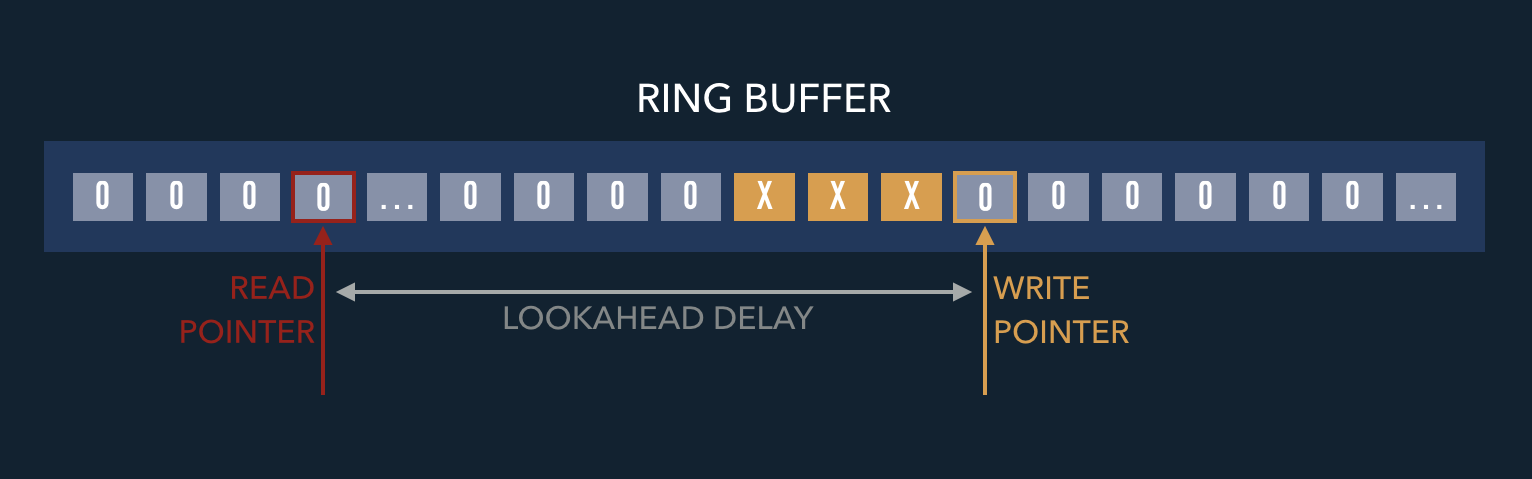
\includegraphics[width=\textwidth]{images/ring_buffer}
\caption{Initialized ring buffer with read and write pointers}
\label{RBuf}
\end{figure}

In principle the implementation of automations is supported by the JUCE framework as well and it can be very simple to implement a standard automation process. The usual case would be a user interacting with the UI and the plug-in communicating these changes to the DAW on write mode. On automation read mode the changes are send back to the plug-in during playback and it does its normal processing chain with changing parameters with the user drawn timing. The study plug-in was a special case and thus, more difficult to realise the automation. In case of the study plug-in the write process of the automation should not be influenced by a user at intended use. Furthermore it should just receive and multiply the adapted gain from the drawn automation at read mode.\\
Like in the Waves plug-in a button was implemented at the UI to switch between read and write mode. Therefore the plug-in always knows if it needs to adapt the gain itself. The read mode implementation was performed quite fast as it just bypasses the regular calculations and multiplies the gain value set by the DAW with the current sample. The communication between DAW and plug-in works well on this part with the predefined parameter class from JUCE.\\
The write mode created more problems: The plug-in adapts the gain value at write mode for every sample. When this would be communicated to the DAW like in normal automation process it has to draw at least 44100 adapted gain values each second. This easily overtaxes a DAW and would be more accurate as it needs to be for a acceptable result. The DAW expects just a few changes per second for the automation as its normal use case (user modifies parameter at UI) would generate. It follows that the drawn automation had to be simplified.\\
At the first attempts automation changes were only communicated when the gain adaption changes its direction (compression/amplification) or when the difference to the last drawn automation point became crucial. With this procedure the output in the DAW would have been acceptable but at some spots it made incorrect jumps. These jumps occured in duration of at most 2 samples but they were still unwanted. Due to involvement of several devices in this process the real cause of the jumps could not be figured out. Different timings and positions for the communication to the DAW and also change of the parameter values were tested until the final solution was found (see chapter \ref{chapter:improvements}.1).\\
There are still jumps in the curve but this is acceptable as the jumps occur rarely and gain difference is about at most 0.1dB. Additionally these jumps are now located at correct positions without smoothing, which is not essential for such small amounts of adaption.\\

\begin{figure}[H]
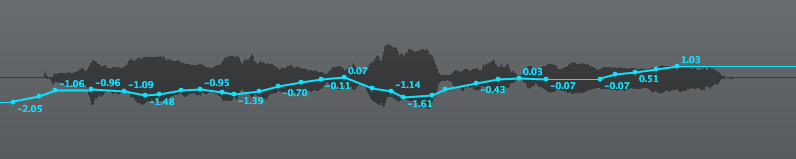
\includegraphics[width=\textwidth]{images/automation}
\caption{Automation written by the study plug-in into a DAW}
\label{auto}
\end{figure}

To simplify the selection of a fitting $L_{goal}$ for a user, a input meter was implemented close to the $L_{goal}$ slider and the current gain adaption. Using this slider it is easier to check whether the current setting works appropriately.\\
Linked on the $L_{goal}$ detection algorithm a button was implemented accessible at the UI which switches the plug-in to $L_{goal}$ detection mode.\\
Side chaining as implemented in chapter \ref{chapter:improvements}.3 is not part of the standard I/O\footnote{I/O = input/output} layout of JUCE but is supported since JUCE version 4.1. To realise another input, it was added in the BusesProperties() structure from the AudioProcessor class. As for the plug-in it is not necessary to have a side chain input, supported bus layouts had not to be changed. Therefore the embedding DAW is able to feed it with a signal but does not need to do so. For further testing in Logic Pro 9\footnote{Logic Pro 9 is DAW developed by Apple} the plug-in had to be revalidated for the DAW, before it accepted the new I/O layout. This was not necessary for previous algorithmic changes.\\
The side chain feature is a addition to the main plug-in but becomes no constant part of it as it is not automatically profitable in every use case. For this reason a button is implemented at the UI to toggle side chain integration on and off. On further term this is useful as different DAWs will handle an undefined (when no input channel/bus is chosen) side chain input in a dissimilar way. For example Logic Pro 9 will send an empty signal containing only zero values. This would effect the outcome of the plug-in when side chain integration is active as it would interpret the signal as a quiet backtrack. With the side chain activation button toggled off by default, there is no urgent need of a silence detection always running in the plug-ins side chain processing chain.\\
As consequence of the idle time being added to the side chain feature the UI was expanded with a pre-gain slider for the side chain input which adds up before the comparison to $L_{goal}$. Controlling the input level of the side chain signal was possible before via a level-controlled bus\footnote{A Bus is a single path for multiple audio sources to be routed and processed.} send but now the mixing engineer is able to do it all at one place while check the level meters for both signals right next to each other at the UI. 

\subsection{Store Settings}

At startup the plug-in regularly initialises with settings that may fit to typical standard cases but always have to be checked and adjusted properly for the current audio tracks. As a mixing engineer could interrupt his/her work, there is need to get its latest settings saved or else it would initialise with the unchanged startup setting. This problem already effects the UI at runtime if it is closed and opened again. Even if the parameters for processing stay correct in this case, the UI could show wrong values at sliders if not correctly refreshed.\\
To prevent this error the getStateInformation() and setStateInformation() which will be called by the DAWs are filled with the necessary save commands.\\

\begin{lstlisting}[frame=single]
void AutoVocalCtrlAudioProcessor::setStateInformation (const 
void* data, int sizeInBytes)
{
    ScopedPointer<XmlElement> xmlState (getXmlFromBinary (data, 
    sizeInBytes));
    if (xmlState != nullptr)
    {
        if (xmlState->hasTagName ("AutoVocalCtrl"))
        {
            *sc = (bool) xmlState
            ->getBoolAttribute ("sc", false);
            *read = (bool) xmlState
            ->getBoolAttribute ("read", false);
           ...
            *loudnessGoal = (float) xmlState
            ->getDoubleAttribute ("loudnessGoal", -20.0);
            *gainRange = (float) xmlState
            ->getDoubleAttribute ("gainRange", 6.0);
            ...
        }
    }
    ...
}
\end{lstlisting}

The plug-in creates a new xml file with the values of all settable parameters in the getStateInformation() method and reads the xml file for parameter adjustment in the setStateInformation() method. Finally the setStateInformation() method notices the UI to refresh the according parameter sliders.\\
As DAWs are calling those methods at different timing but always at startup and before the shutdown of the plug-in or the UI, all user-made made adjustments are saved and regained at startup. Additional this procedure could save and regain presets for the plug-in which can be used in other mixing session for example as orientation for the parameter adjustment.\\

\subsection{UI Design}

The main focus of this study was the algorithm behind the plug-in. Nevertheless it was the intension that a user should be able to work with the plug-in without reading a manual. Therefore the JUCE dummy UI was refactored after parameter reduction.\\
The main problem of the previous UI was the lack of the possibility to differ between sliders for parameter adjustments and elements which were displaying inside information of the plug-in (see Fig. \ref{UIold}). Furthermore, the slider labels and value indicators were too small to display in complete length, while additionally confusing by their large number.\\

\begin{figure}[H]
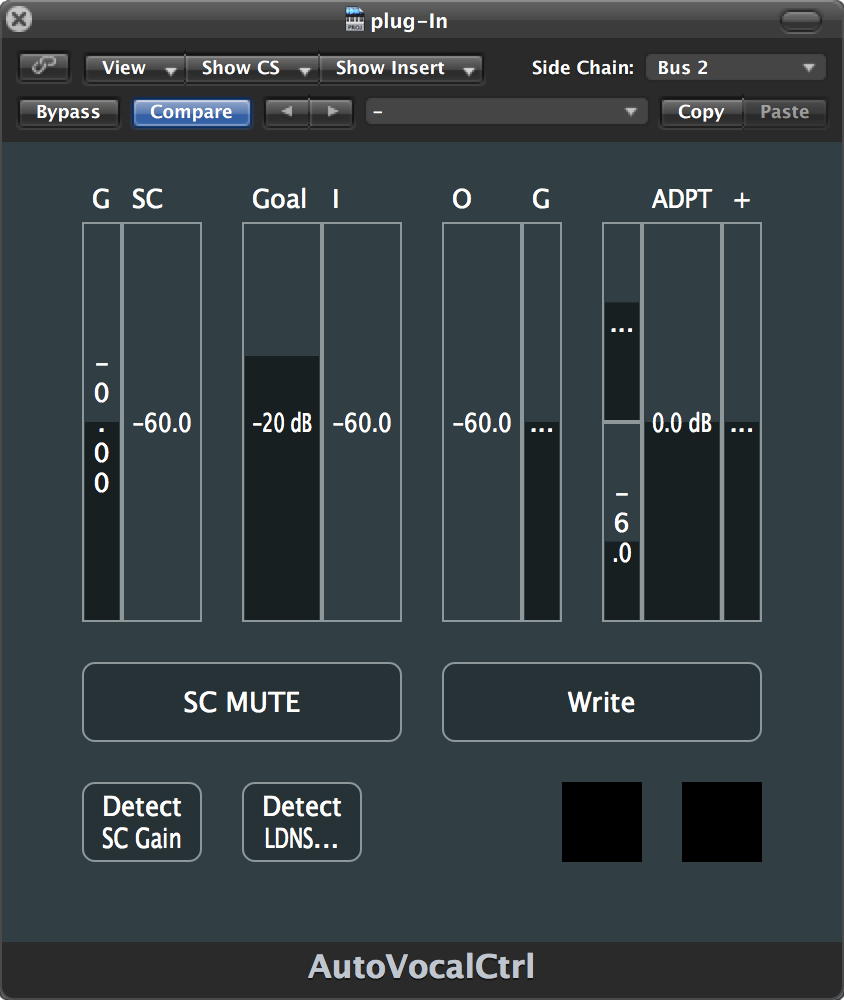
\includegraphics[width=0.5\textwidth]{images/designVorher}
	\centering
	\caption{UI after parameter reduction}
	\label{UIold}
\end{figure}

The main challenge in the UI re-design was highlighting of usable elements. To differentiate from only informational parts, all the changeable components are coloured red. The colour is chosen as it strongly diverges from its complementary colour green which is the plug-in’s main colour (see Fig. \ref{UInew}). Additionally only the usable sliders and buttons got a coloured frame instead of the plain black outline of the pure metering components.\\

\begin{figure}[H]
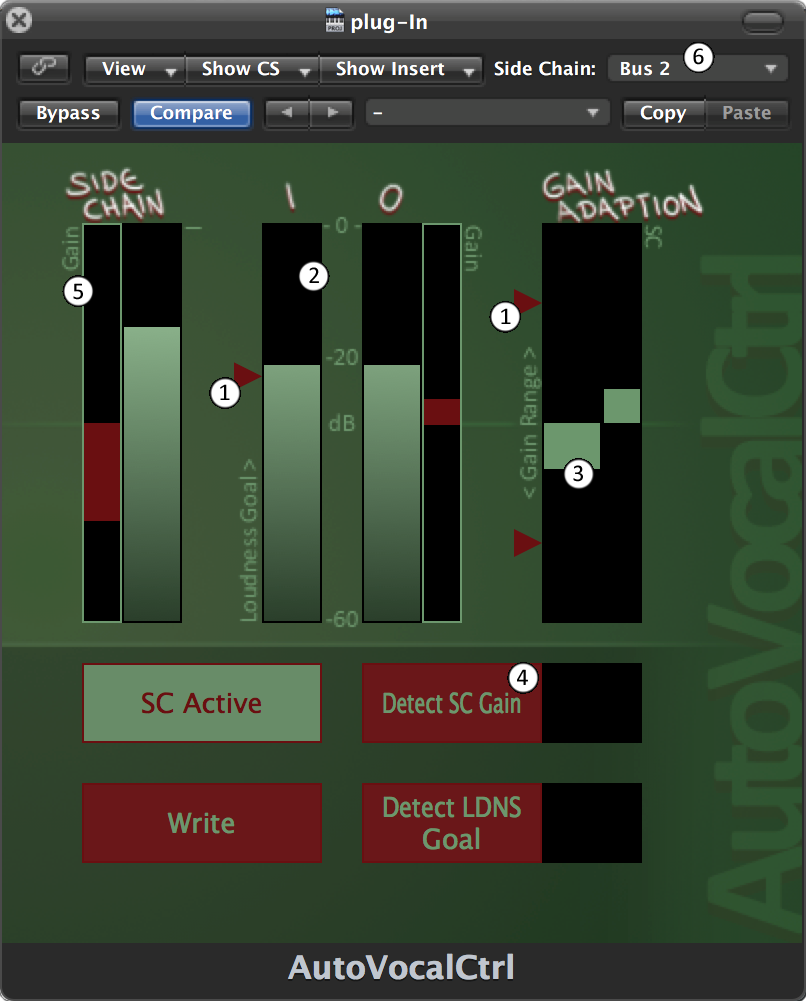
\includegraphics[width=0.5\textwidth]{images/designNeuNum}
	\centering
	\caption{Final UI in Logic Pro 9}
	\label{UInew}
\end{figure}

In the new design the gain range and loudness goal are set via red triangles ((1) in Fig. \ref{UInew}) pointing on the corresponding level/gain meter. This was done to let the user recognize the connection between these UI elements. $L_{goal}$ should be set in consideration of the input level meter (2) right next to it and the gain range is directly modifying the maximal and minimal values of the connected gain reduction meter (3).\\
The three meters which are displaying the I/O levels (input, side chain input, output) are next to each other and visualising their value with a rising bar where a colour gradient is applied to. Therefore the green tone of the bar is getting brighter with increasing signal level to support a fast assessment of the user.\\
All UI elements excluding the buttons are divided in different sections: The I (input), O (output), side chain and gain adaption section, containing the related components. To indicate which task the single components fulfil, they have an additional label, on the side which is not adjoining to another UI element.\\
When the Side Chain feature is disabled, the corresponding gain detection button (4) and the side chain input gain slider (5) become disabled too, as they would have no effect. This can be recognized by the user as the red colour of these UI elements gets greyer and the slider loses its green frame which previously signalled a possible interaction. The components which only display information are disabled for user interaction by default.\\
For most of the slider elements it is not necessary for the user to know the exact value but to get an approximation and therefore a feeling about what is happening. Clear slider values often seduce users to adjust sliders to pretty numbers (e.g. rounding to 5 or repeated digits) instead of only observing the change of the outcome. As consequence most of the slider values are removed in the new design. An orientation for the input and output meters is still located next to them but in a light green like the element labels in order to not distract from the main information.\\
The side chain input (6) is chosen in the embedding DAW and therefore not to set in the plug-in’s UI.\\

\section{Test Environment}

The JUCE framework allows two ways to run the plug-in. The fastest way is to build the plug-in as standalone application which can be done directly from the IDE\footnote{integrated development environment}. The plug-in is starting directly and the main input and output channels could be chosen. This is well suited for testing for small bug fixes or visual changes. The standalone procedure has its limitation in terms of e.g. a side chain input as it is not embedded in an surrounding DAW. For this case JUCE offers the Audio Plugin Host as solution. The Audio Plugin Host can host different plug-ins simultaneously and visualises all inputs and outputs. It is enabling connections between I/0 ports and the currently active audio interface of the operating computer. The advantage compared to a real DAW is that debugging output is provided during runtime.\\
It was necessary to test the plug-in in a real DAW for a realistic environment and to use all considered features, for instance writing an automation or comfortably feeding a real backtrack into the side chain input. Logic Pro 9 was used to run the study plug-in for the reason that it works with AU plug-ins which are per default supported by JUCE. Using the custom UI it was still possible to change calculation parameters at runtime.\\
For tests inside the DAW professional recorded audio tracks are needed additionally. For testing side chain adaption it was necessary to work with full musical compositions and not only to remain on vocal pieces. Therefore fitting multitrack projects from an online library\cite{MultiT} of free educational use were utilized (same projects as used in side chain evaluation, chapter \ref{chapter:evaluation}).\\
Before all features came together, basic algorithmic tests were performed. Python was used because of its simplicity and helpful visual features. Therefore different approaches could be tested efficiently and visualised whether they have performed their task correctly.\\
